\chapter{Divide Areas Algorithm}
\label{chp:DARP}

\section{Background Theory}
Grid-based coverage path planning can be implemented using a number of different methods.\\
Naturally, achieving the most optimal solution possible would be most desirable. The authors of \cite{DARP2017} propose a set of requirements for optimal coverage path planning using a grid-based approach. These fundamental conditions, as they call them, are listed below.
\begin{enumerate}
	\item Every cell in the environment, that is not classified as an object, must be covered. This is known as complete coverage.
	\item Each cell in the environment must only be searched once, and only by one of the robots. This is known as the non-backtracking requirement.
	\item Each robot should have as close to an equal amount of cells as possible assigned to it for searching. Their sets of cells should be of roughly the same size.
	\item The sets of cells assigned to each robot should be a connected sub-region. This means that when generating a path to search the cells within its set, a robot would not need to traverse that of another to search it's own sub-region.
	\item The initial position of each robot should be contained within the set of cells assigned to it. This means that a robot would not need to traverse another robot's sub-region to reach its sub-region for searching.
\end{enumerate}
The authors developed a methodology to achieve these conditions of optimality. They called it The \acf{darp}. Their solution seeks to divide a known environment containing static obstacles into contiguous sub-regions. These regions are formed based on the robot starting positions so that each robot starts within one of the regions.\\ 
The solution is found in an iterative manner and it converges to where the sub-regions are cohesive and roughly the same size. \acs{darp} only divides the region appropriately between robots. A single robot \acs{cpp} algorithm can then be utilised to achieve complete coverage of each sub-region, which translates to complete coverage of the whole environment.
% TODO: Maybe mention something about the EXISTENCE of solutions
% Coverage
% Grid Based
% Optimize
\subsection{Algorithm Description}
\begin{figure}[h!]
	\centering
	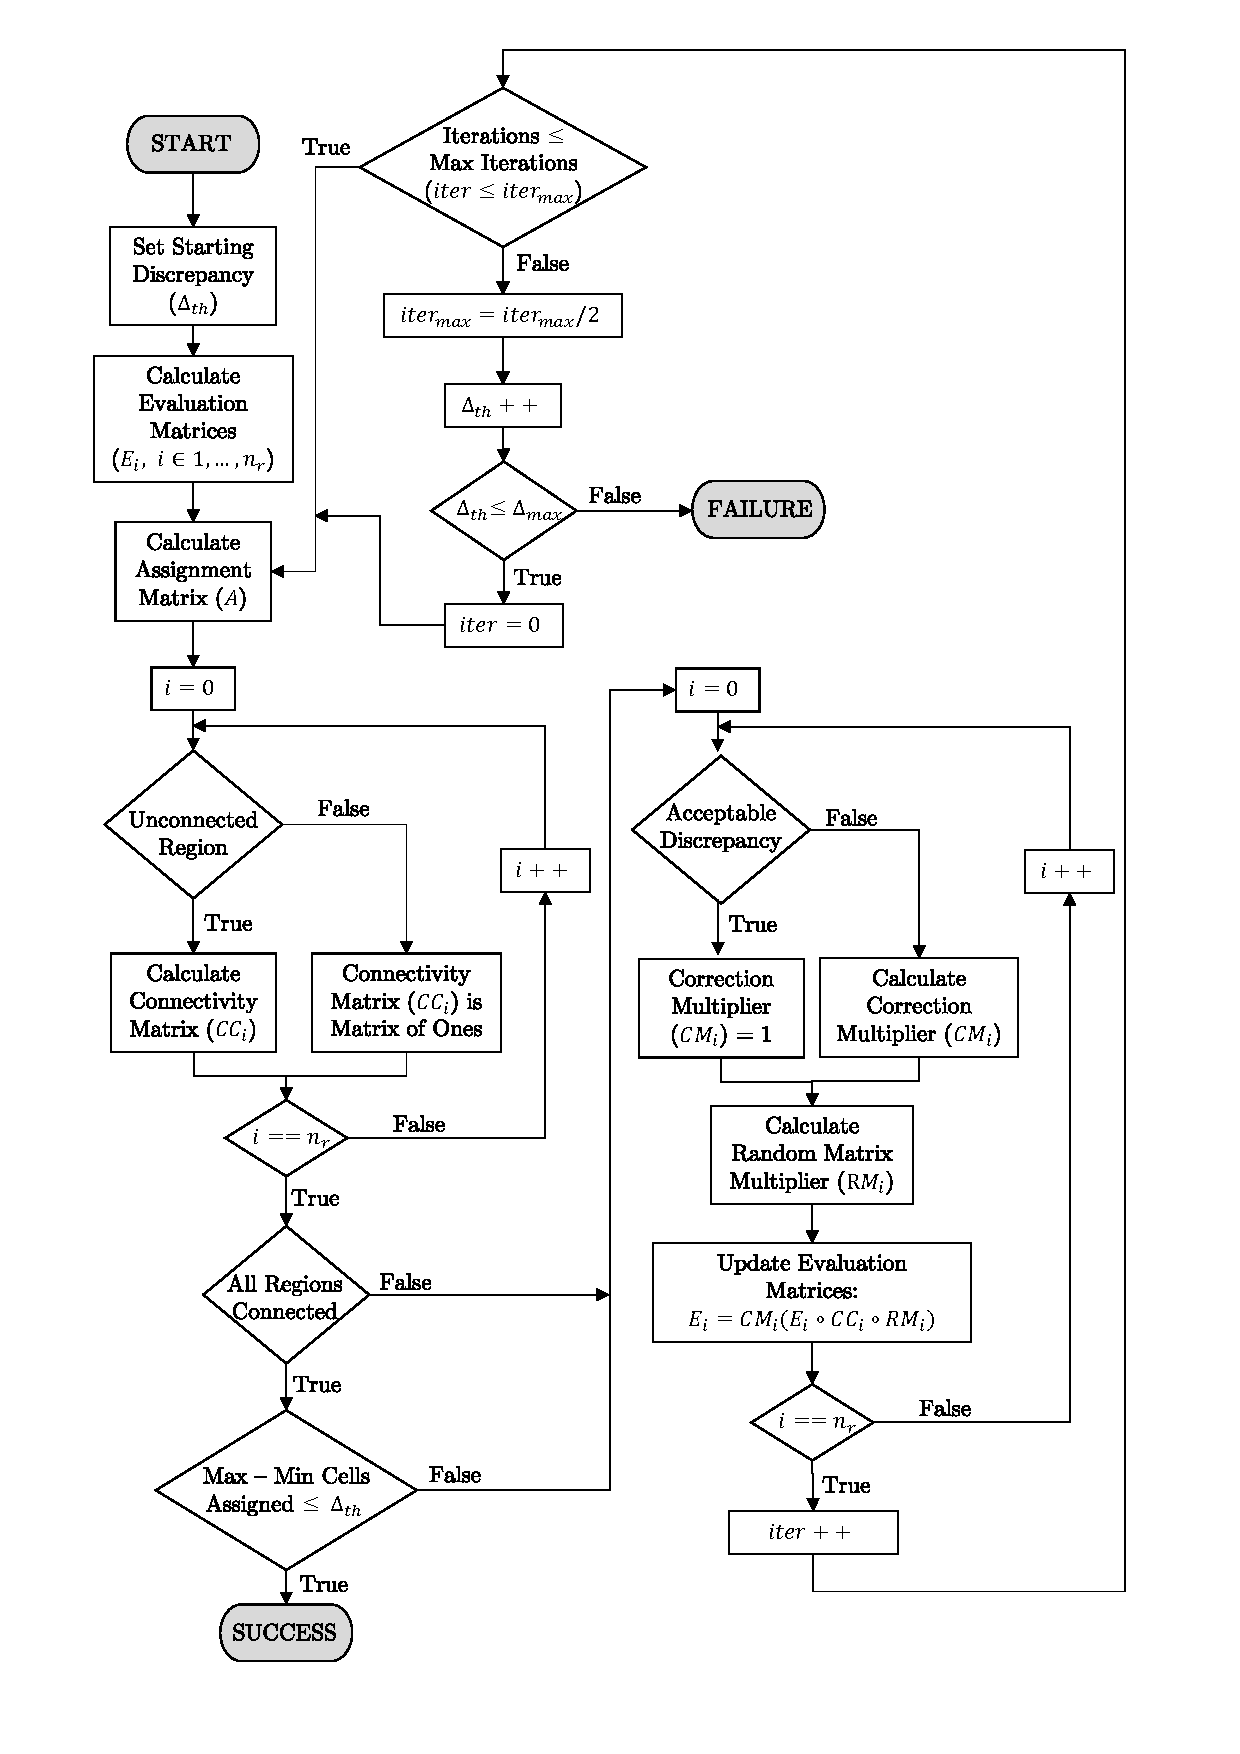
\includegraphics[scale=0.8,trim={1.5cm 0 1.5cm 0},clip]{figs/DARP_Diagram3.pdf}
	\caption{Flow diagram representing the logic for DARP.}
	\label{fig:DARP}
\end{figure}

\section{Distance Measure Comparisons}

\section{Implementation with Different Environments}